% Yesternity: Bias Bounty Mapping Equity Challenge writeup (Best Bias Discovery + Best Documentation).
% Build:  cd docs/paper && pdflatex paper.tex && pdflatex paper.tex   (figures first: python src/paper_figures.py)
\documentclass[10pt,twocolumn,a4paper]{article}
\usepackage[T1]{fontenc}
\usepackage{mathptmx}
\usepackage[scaled=0.90]{helvet}
\usepackage{courier}
\usepackage[a4paper,top=19mm,bottom=21mm,left=17mm,right=17mm,columnsep=7mm]{geometry}
\usepackage[hyphens]{url}
\usepackage{graphicx,booktabs,tabularx,array,amsmath,enumitem,float,needspace}
\usepackage[dvipsnames]{xcolor}
\usepackage[protrusion=true,expansion=true]{microtype}
\DisableLigatures[-]{encoding=*,family=tt*}      % keep the two hyphens of --strata and --geometry in copied commands
\usepackage[font=small,labelfont=bf,skip=6pt]{caption}
\usepackage{titlesec,fancyhdr}
\usepackage[most]{tcolorbox}
\definecolor{accent}{HTML}{2A78D6}
\definecolor{once}{HTML}{EB6834}
\definecolor{ink2}{HTML}{52514E}
\usepackage[colorlinks=true,linkcolor=accent,urlcolor=accent,citecolor=accent,pdfborder={0 0 0}]{hyperref}
\hypersetup{pdftitle={Phantom Road Gaps: reference bookkeeping makes up most of the road-coverage gap, and it bends the scorecard built to reveal inequity},
            pdfauthor={Team Yesternity (ahammadshawki8, ahnafjamil, Ashfaqul_Hasan)},
            bookmarksopen=true,bookmarksnumbered=true,pdfpagemode=UseOutlines}

% the two selected finals, in one place
\newcommand{\finalAid}{EVGrZBHt}\newcommand{\finalAname}{E134}\newcommand{\finalAscore}{0.05556589}
\newcommand{\finalBid}{E3u62GkV}\newcommand{\finalBname}{E136}\newcommand{\finalBscore}{0.055506023}

\titleformat{\section}{\normalfont\large\bfseries}{\thesection}{0.55em}{}
\titleformat{\subsection}{\normalfont\normalsize\bfseries}{\thesubsection}{0.5em}{}
\titleformat{\paragraph}[runin]{\normalfont\normalsize\bfseries}{}{0pt}{}[.]
\titlespacing*{\section}{0pt}{15pt plus 4pt minus 2pt}{6pt plus 1pt}
\titlespacing*{\subsection}{0pt}{11pt plus 3pt minus 1pt}{4pt plus 1pt}
\titlespacing*{\paragraph}{0pt}{6pt plus 2pt}{0.6em}
% a heading never starts with too little room left in its column: it moves to the next one instead
\let\origsection\section\renewcommand{\section}{\Needspace{9\baselineskip}\origsection}
\let\origsubsection\subsection\renewcommand{\subsection}{\Needspace{6\baselineskip}\origsubsection}
\let\origparagraph\paragraph\renewcommand{\paragraph}{\Needspace{4\baselineskip}\origparagraph}
\setlist{itemsep=1.5pt,topsep=4pt,parsep=0pt,leftmargin=1.3em}
\setlength{\parskip}{2pt plus 1pt}
\linespread{1.03}
\raggedbottom
\widowpenalty=10000 \clubpenalty=10000                  % no lone line at the top or foot of a column
\setlength{\textfloatsep}{16pt plus 4pt minus 3pt}
\setlength{\floatsep}{14pt plus 3pt minus 2pt}
\setlength{\dbltextfloatsep}{18pt plus 4pt minus 3pt}
\setlength{\dblfloatsep}{14pt plus 3pt minus 2pt}
\setlength{\intextsep}{12pt plus 3pt minus 2pt}
\renewcommand{\arraystretch}{1.18}
\setlength{\tabcolsep}{4pt}
\newcolumntype{L}{>{\raggedright\arraybackslash}X}
\newcolumntype{R}{>{\raggedleft\arraybackslash}X}
\pagestyle{fancy}\fancyhf{}
\fancyhead[L]{\footnotesize\color{ink2}Team Yesternity \textperiodcentered{} Bias Bounty Mapping Equity Challenge}
\fancyhead[R]{\footnotesize\color{ink2}Best Bias Discovery \& Best Documentation}
\fancyfoot[C]{\footnotesize\color{ink2}\thepage}
\renewcommand{\headrulewidth}{0.3pt}
\newcommand{\partbanner}[2]{%                     banner, kept on the same column as the criteria box after it
  \par\Needspace{14\baselineskip}\vspace{6pt}\noindent
  \colorbox{#1}{\parbox{\dimexpr\columnwidth-2\fboxsep}{\color{white}\bfseries\strut #2}}\par\nopagebreak\vspace{2pt}}
\newcommand{\code}[1]{\texttt{\small #1}}
% every figure and table sits in a thin frame, caption included, so it stands apart from the text
\tcbset{floatframe/.style={enhanced,nobeforeafter,colback=white,colframe=ink2!30,boxrule=0.4pt,arc=1mm,boxsep=0pt,
  left=4pt,right=4pt,top=4pt,bottom=4pt}}
\makeatletter
\let\pg@endfloatbox\@endfloatbox
\renewcommand{\@endfloatbox}{\pg@endfloatbox
  \global\setbox\@currbox\vbox{\moveleft4.4pt\hbox{\tcbox[floatframe]{\box\@currbox}}}}
\makeatother
\newtcolorbox{figpanel}{floatframe,equal height group=figrow}

\begin{document}
\twocolumn[{%
\begin{center}
{\fontsize{24}{28}\selectfont\bfseries Phantom Road Gaps\par}
\vspace{5pt}
{\large\itshape Reference bookkeeping makes up most of the road-coverage gap,\\[1pt]
and it bends the scorecard built to reveal inequity\par}
\vspace{8pt}
{\large Team Yesternity\par}
\vspace{2pt}
{\normalsize Shawki (Zindi: \code{ahammadshawki8})\quad\textperiodcentered\quad Ahnaf (Zindi: \code{ahnafjamil})\quad\textperiodcentered\quad
Ashfaq (Zindi: \code{Ashfaqul\_Hasan})\par}
\vspace{3pt}
{\small\color{ink2} 1 November 2026\quad\textperiodcentered\quad Code: \url{https://github.com/ahammadshawki8/phantom-road-gaps}\par}
\end{center}
\vspace{-9pt}
\begin{tcolorbox}[enhanced,colback=accent!6,colframe=accent,boxrule=0.6pt,arc=1.5mm,left=2.5mm,right=2.5mm,top=1.2mm,bottom=1.2mm]
\small\textbf{Entered for:} Best Bias Discovery (Part~A) and Best Documentation (Part~B).\quad
\textbf{Leaderboard submissions this writeup describes:} \code{\finalAid} (\finalAname, public RMSE \finalAscore, private 0.056132715) and
\code{\finalBid} (\finalBname, public RMSE \finalBscore, private 0.05613082), our two selected finals. Both are built only from the challenge package.
\end{tcolorbox}
\vspace{1pt}
\begin{tcolorbox}[enhanced,colback=white,colframe=white,boxrule=0pt,left=6mm,right=6mm,top=0mm,bottom=0mm]
\small\noindent\textbf{Abstract.}
The Bias Bounty coverage-gap score compares Overture's map of each census tract with hidden reference layers, and a
scorecard then compares the score across rural, tribal, vulnerable and hazard-exposed places. We show that the road part
of the score mostly measures how the reference is counted, and that this bends the scorecard itself. Two counting rules
do it: a highway along a tract boundary is counted in full in both tracts, and a
stretch that carries two route numbers or a second name is counted again. Measured from the challenge package alone and
tested against the hidden scores, they make up 72\% of the mean road gap of the 6,593 road-scored tracts (55--80\% across
every weighting we tried; 0.23 is added in urban Oklahoma, 0.07 in urban Arizona). Counted once, the rural-to-urban ratio
of the score rises from 2.34 to 2.73 and the wildfire-hazard ratio from 1.67 to 1.81, while the social-vulnerability ratio
falls from 1.16 to 1.01: the reported disadvantage of rural and fire-exposed places is understated, and nearly all of the
reported social-vulnerability disparity is bookkeeping. On a worklist of the 660 worst-scored tracts, 321 are there for
highways already on the map, and the 321 they push off it are 71\% rural, 58\% tribal and 83\% above the median wildfire
hazard. Public Census and FEMA data agree: those 321 have 1.8 times the share of mobile homes of the tracts that crowd them
out, and FEMA rates three times as many high for wildfire risk. Every number is recomputed by a named script; 33 are
checked in a second from a few megabytes.
\end{tcolorbox}
\vspace{1pt}
\begin{tcolorbox}[enhanced,colback=once!7,colframe=once,boxrule=0.6pt,arc=1.5mm,left=2.5mm,right=2.5mm,top=1mm,bottom=1mm,
  title={\small\bfseries The finding in four numbers},coltitle=white,colbacktitle=once,fonttitle=\small\bfseries,
  toptitle=0.3mm,bottomtitle=0.3mm]
\small
\begin{tabularx}{\linewidth}{@{}>{\raggedright\arraybackslash}X>{\raggedright\arraybackslash}X>{\raggedright\arraybackslash}X>{\raggedright\arraybackslash}X@{}}
\textbf{72\%} of the mean road gap is bookkeeping, not missing roads (55--80\% under any weighting; Sec.~\ref{sec:evidence}). &
\textbf{2.34 $\rightarrow$ 2.73}: the scorecard's rural ratio counted once; social vulnerability 1.16 $\rightarrow$ 1.01 (Fig.~\ref{fig:scorecard}). &
\textbf{321 of 660} worst-scored tracts are on the list for highways that are mapped already (Fig.~\ref{fig:worklist}). &
\textbf{71\% rural, 58\% tribal}: the 321 tracts the bookkeeping pushes off that list (Table~\ref{tab:hidden}).
\end{tabularx}
\end{tcolorbox}
\vspace{3pt}
\noindent\begin{minipage}[t]{0.485\textwidth}
\begin{figpanel}
\centering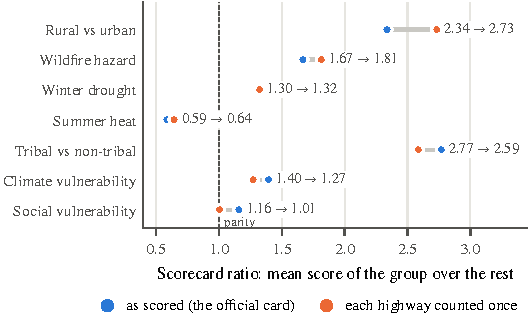
\includegraphics[width=\linewidth]{p8_scorecard.pdf}
\captionof{figure}{The scorecard on our final, as scored (the card the leaderboard prints) and counted once: rural
and wildfire disadvantage is understated; the social-vulnerability gap is mostly bookkeeping (\S\ref{sec:scorecard}).}
\label{fig:scorecard}
\end{figpanel}
\end{minipage}\hfill
\begin{minipage}[t]{0.485\textwidth}
\begin{figpanel}
\centering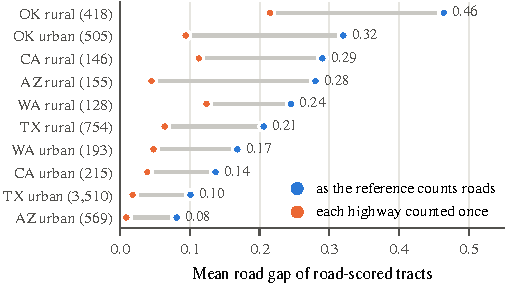
\includegraphics[width=\linewidth]{p1_gap_by_region.pdf}
\captionof{figure}{Bookkeeping makes up most of the road gap in every region and urbanity, far more in Oklahoma than
in Arizona or Texas (tracts per row in brackets; \S\ref{sec:evidence}).}
\label{fig:gap}
\end{figpanel}
\end{minipage}
\vspace{3pt}

\noindent\begin{minipage}[t]{0.485\textwidth}
\begin{tcolorbox}[enhanced,equal height group=criteria,colback=accent!5,colframe=accent!60,boxrule=0.4pt,arc=1mm,left=1.5mm,right=1.5mm,top=0.8mm,bottom=0.8mm,
  title={\footnotesize\bfseries Part A, Best Bias Discovery: where each criterion is answered},coltitle=white,
  colbacktitle=accent,toptitle=0.2mm,bottomtitle=0.2mm]
\footnotesize
\textbf{Novelty} \S\ref{sec:pattern}, \S\ref{sec:scorecard}: a pattern outside the grid that bends the grid.
\textbf{Evidence} \S\ref{sec:evidence}: lengths, tests on the hidden scores, robustness, named tracts, a worked example.
\textbf{Impact} \S\ref{sec:affected}: understated disadvantage, a distorted worklist, evacuation, Census and FEMA data (\S\ref{sec:outside}).
\textbf{Reproducibility} \S\ref{sec:reproA}: 33 checks in a second; Appendix~\ref{app:repro}.
\textbf{Also:} limits \S\ref{sec:limits}, fix \S\ref{sec:fix}, prior work \S\ref{sec:prior}.
\end{tcolorbox}
\end{minipage}\hfill
\begin{minipage}[t]{0.485\textwidth}
\begin{tcolorbox}[enhanced,equal height group=criteria,colback=once!5,colframe=once!60,boxrule=0.4pt,arc=1mm,left=1.5mm,right=1.5mm,top=0.8mm,bottom=0.8mm,
  title={\footnotesize\bfseries Part B, Best Documentation: the organisers' checklist},coltitle=white,
  colbacktitle=once,toptitle=0.2mm,bottomtitle=0.2mm]
\footnotesize
\textbf{Overview:} \S\ref{sec:overview}.
\textbf{Data sources:} \S\ref{sec:data}.
\textbf{How each component was computed:} \S\ref{sec:components}.
\textbf{Edge cases} (zero-population, water-dominated, data-sparse): \S\ref{sec:edge}, Table~\ref{tab:edge}.
\textbf{Alternative weightings and why:} \S\ref{sec:weights}, Table~\ref{tab:weights}.
\textbf{Reproducibility:} \S\ref{sec:repro}, Appendix~\ref{app:repro}; both finals rebuild from the package to
$3\times10^{-16}$.
\end{tcolorbox}
\end{minipage}
}]
\clearpage

\section{Introduction}
\label{sec:intro}
The challenge scores each census tract by how much of a reference map Overture lacks. For roads, it compares the length of
Overture's highway-class roads inside the tract with the length of primary and secondary road in Census TIGER/Line (codes
S1100 and S1200~\cite{mtfcc}). The organisers' scorecard then compares these gaps across urban and rural tracts, tribal
land, social and climate vulnerability and hazard exposure~\cite{zindi}.

We show that the road part of that score mostly measures how the reference is counted, not how much of the highway network
is missing, and that this distorts the very comparisons the scorecard exists to make. Our contributions:
\begin{enumerate}
\item \textbf{The size of the bookkeeping}: two counting rules from public challenge discussion (\S\ref{sec:prior}),
measured here from the package alone and tested against the hidden scores, make up 72\% of the mean road gap (55--80\%
under any weighting), from 0.07 in urban Arizona to 0.23 in urban Oklahoma (\S\ref{sec:pattern}--\ref{sec:evidence}).
\item \textbf{The scorecard it bends}: removing it raises the rural and wildfire-hazard ratios by 17\% and 9\% and
removes nearly all of the social-vulnerability disparity (\S\ref{sec:scorecard}).
\item \textbf{The places it hides}: a worst-tenth worklist holds 321 tracts whose highways are mapped and leaves out 321
that are mostly rural, tribal and fire-exposed; we name examples on both sides (\S\ref{sec:affected}), and public Census
and FEMA data show the hidden places are older, less connected and at higher risk (\S\ref{sec:outside}).
\item \textbf{A check anyone can run}: 33 of the paper's numbers recomputed in under a second from a few megabytes of the
package, and a label-free method whose finals rebuild to within $3\times10^{-16}$ (\S\ref{sec:reproA}, Part~B).
\end{enumerate}

\partbanner{accent}{Part A \quad Best Bias Discovery}

\section{The pattern the scorecard does not surface}
\label{sec:pattern}
\textbf{In one sentence: the road score counts a highway on a tract boundary in both tracts, and counts a highway once
per route number and per name, so much of what it reports as missing road is bookkeeping.}


The organisers' formula cuts both road layers with the tract polygons by an overlay intersection~\cite{readme}. We call
the reference length a tract receives this way its \emph{bookkept reference length}, and split it into three parts that can
be measured from the package alone:
\begin{enumerate}
\item \textbf{Interior highway}: highway that runs through the tract, measured as the length of Overture road inside the
tract that carries an Interstate, US or state route number.
\item \textbf{Boundary highway}: highway whose centreline is the tract boundary. Census tract boundaries follow visible
features~\cite{garm}, most often roads, so the boundary polyline in the package's tract file is the reference's own
highway line, and the overlay counts it inside both tracts. We sample every tract boundary every 10~m and match each
sample to the nearest Overture route within a region-specific distance (Table~\ref{tab:regions}); a stretch is counted
when Overture's copy lies outside the tract.
\item \textbf{Duplicate records}: extra records on the same stretch. The reference holds one record per route number and
per name, so where two routes share a road, or a route also carries a local street name or an honorific highway name,
the same metres are counted again. We count the extra route numbers and names on each stretch from Overture's own route
and name attributes.
\end{enumerate}
A tract follows the pattern when parts 2 and 3 are a large share of its reference length, or when they change its road
gap by a large amount.

\subsection{Why the scorecard cannot see it}
The automated scorecard takes each tract's road gap as given and compares averages across fixed groups: urbanity, social and climate
vulnerability, tribal land and hazards. It never asks what the reference length inside a tract consists of. A boundary
highway counted on both sides, and a stretch counted once per name, look to it exactly like highway that Overture is
missing. The pattern is a data-source behaviour of the reference, not of Overture, and it depends on region and on where a
tract's highway runs relative to its boundary, so no split by the scorecard's strata can separate it from real coverage.
It is the kind of discovery the challenge describes as ``a data source behavior''. Worse, because the bookkeeping is
uneven across places, it shifts the scorecard's own ratios: it is a pattern outside the grid that bends the grid
(Section~\ref{sec:scorecard}).

\section{The evidence}
\label{sec:evidence}
\subsection{Bookkeeping is almost half of the reference length}
Over all tracts, the package shows 102,551~km of route-numbered highway inside tracts, 16,759~km of boundary highway whose
Overture copy lies outside the tract, and 71,937~km of extra route and name records (Table~\ref{tab:regions}). Overture's
side also contains 12,448~km of motorway ramps that the reference's road classes leave out. At face value, boundary
highway and duplicate records are 46\% of the bookkept reference length.

\begin{table}[t]
\centering\small
\caption{What the reference counts, by region. The distance cut is the furthest a boundary sample may sit from Overture's
highway and still be read as that highway, fitted per region by maximum likelihood from the boundary-to-highway
distances, with no reference to the score. Interior: route-numbered highway inside tracts. Boundary: boundary highway whose
Overture copy lies outside the tract. Extra records: length of additional route numbers and names.}
\label{tab:regions}
\setlength{\tabcolsep}{2pt}\footnotesize
\begin{tabular*}{\columnwidth}{@{\extracolsep{\fill}}lrrrrr@{}}
\toprule
 & Road-scored & Cut & Interior & Boundary & Extra\\
Region & tracts & (m) & (km) & (km) & records (km)\\
\midrule
Oklahoma   & 923   & 21.4 & 24,293 & 2,849 & 20,095\\
Texas      & 4,264 & 19.2 & 51,710 & 9,810 & 30,168\\
Arizona    & 724   & 15.8 & 11,422 & 2,288 & 13,805\\
Washington & 321   & 11.3 & 8,142  & 832   & 3,741\\
California & 361   & 10.6 & 6,984  & 980   & 4,127\\
\bottomrule
\end{tabular*}
\end{table}

The distance cut itself differs by region. In Oklahoma and Texas the gap between the tract line and Overture's highway has
a long tail and the cut sits near 20~m; in California and Washington it is near 11~m. So the same highway geometry is
matched differently in different regions, and that is visible in the package without any model.

\subsection{Each counting rule was tested against the hidden scores}
\label{sec:tests}
We do not have to assume that the reference behaves this way. Each rule was added to our model as a single change and
submitted once, and the change in the public score measures how strongly the change agrees with the hidden target
(Section~\ref{sec:weights} gives the arithmetic; zero means no agreement, and one standard error is about 0.02).
Every rule raised the score, by 2 to 24 standard errors (Figure~\ref{fig:agreement}).

\begin{figure}[t]
\centering
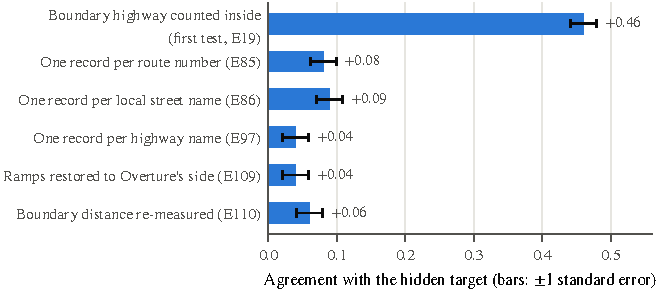
\includegraphics[width=\columnwidth]{p4_agreement.pdf}
\caption{Each counting rule's agreement with the hidden target, read from the change in public score when it was added
alone. Bars are $\pm1$ standard error of the public sample.}
\label{fig:agreement}
\end{figure}

The boundary rule is the largest single effect we measured in the whole competition. When we later fitted the model's
weights to everything the leaderboard had revealed, the boundary highway kept a weight of 0.92 and each extra record about
0.53 to 0.55: the reference counts boundary highways almost fully, and each duplicate name about half the time. Every
number in the rest of Part~A uses these fitted weights, not the face-value counts.

\subsection{Bookkeeping adds 0.07 to 0.23 to the road gap, unevenly by region}
To turn lengths into a road gap we use our calibrated simulator (Section~\ref{sec:components}): it draws the hidden
reference for each tract many times and averages the resulting gap. Its road part is the one tested in
Figure~\ref{fig:agreement}. We run it twice with the same calibration: once as the reference counts, and once with the
boundary and duplicate-record terms switched off, so each highway counts once, in the tract it runs through. The
difference is the road gap that the bookkeeping adds (Figure~\ref{fig:gap}, Table~\ref{tab:urbanity}).

\begin{table}[t]
\centering\small
\caption{Mean road gap of road-scored tracts (0: the map has all of the reference's highway; 1: none). Urban and rural
follow the Rural-Urban Commuting Area code (rural is code 4 or above).}
\label{tab:urbanity}
\begin{tabularx}{\columnwidth}{@{}lRRRR@{}}
\toprule
 & \multicolumn{2}{c}{Urban} & \multicolumn{2}{c}{Rural}\\
\cmidrule(lr){2-3}\cmidrule(l){4-5}
Region & as scored & counted once & as scored & counted once\\
\midrule
Oklahoma   & 0.32 & 0.09 & 0.46 & 0.22\\
Arizona    & 0.08 & 0.01 & 0.28 & 0.05\\
Texas      & 0.10 & 0.02 & 0.21 & 0.06\\
California & 0.14 & 0.04 & 0.29 & 0.11\\
Washington & 0.17 & 0.05 & 0.25 & 0.12\\
\bottomrule
\end{tabularx}
\end{table}

The comparison is within region and within urbanity, so it is not the urban/rural or regional split that the scorecard
already shows. The bookkeeping adds 0.23 in urban Oklahoma (95\% bootstrap interval 0.21--0.24), 0.12 in urban
Washington, 0.10 in urban California, 0.08 in urban Texas (0.079--0.088) and 0.07 in urban Arizona (0.06--0.08). Rural
tracts show the same ordering. Of the two parts, the duplicates add more in every region; the boundary part is largest in
rural Arizona (0.08 on its own). Figure~\ref{fig:map} shows where it falls inside Oklahoma, the region where it is
largest.

\subsection{The headline does not depend on the fitted weights}
The 72\% uses the weights the hidden scores chose (boundary 0.92, duplicate records about 0.54). Table~\ref{tab:sens}
runs the same calibrated simulator with other weights. Counting every record in full gives 80\%; halving both weights
still gives 55\%; the duplicate rule alone gives 62\% and the boundary rule alone 46\%. So ``most of the road gap'' holds
under every weighting except one rule on its own, and the ordering of regions does not change
(\code{writeup\_numbers.py sensitivity}).

\begin{table}[t]
\centering\small
\caption{Share of the mean road gap of road-scored tracts that is bookkeeping, under different counting weights (same
calibration; counted once, the mean road gap is 0.047 in every row).}
\label{tab:sens}
\begin{tabular*}{\columnwidth}{@{\extracolsep{\fill}}lrrr@{}}
\toprule
Weights & Boundary & Duplicates & Share\\
\midrule
Fitted (used in this paper) & 0.92 & $\times$1.00 & \textbf{72\%}\\
Every record in full & 1.00 & $\times$1.81 & 80\%\\
Half of the fitted & 0.46 & $\times$0.50 & 55\%\\
Duplicate rule alone & 0 & $\times$1.00 & 62\%\\
Boundary rule alone & 0.92 & 0 & 46\%\\
\bottomrule
\end{tabular*}
\end{table}

\begin{figure}[t]
\centering
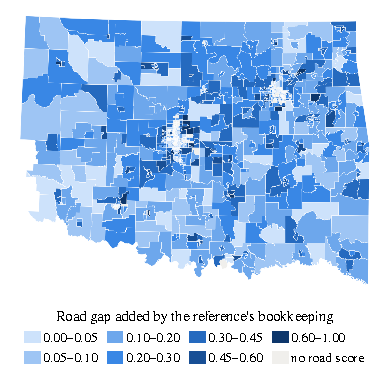
\includegraphics[width=\columnwidth]{p3_map_oklahoma.pdf}
\caption{Road gap added by the reference's bookkeeping, eastern Oklahoma. It is largest in the Oklahoma City and Tulsa
metro tracts, where highways run on tract lines and carry several route numbers and names.}
\label{fig:map}
\end{figure}

\subsection{It changes which tracts look worst}
Ranked by road gap, 660 tracts form the worst tenth. With each highway counted once, 321 of them (49\%) fall out of that
tenth (Figure~\ref{fig:worklist}). They hold 507,345 homes and 1.19 million people. Over the whole map, 1,548 tracts get
at least 0.2 of their road gap from bookkeeping; they hold 2.5 million homes and 5.8 million people.

\begin{figure}[t]
\centering
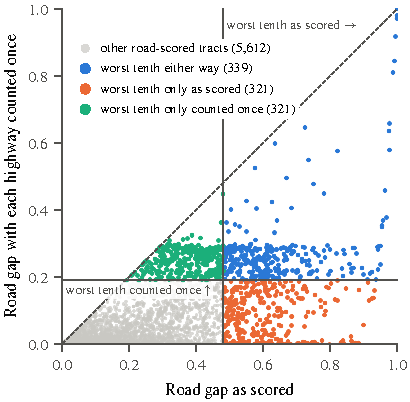
\includegraphics[width=\columnwidth]{p5_worklist.pdf}
\caption{Every road-scored tract, as scored against counted once. Orange tracts are in the worst tenth only because of
the bookkeeping: 321 of the 660 worst-scored tracts.}
\label{fig:worklist}
\end{figure}

\subsection{Ten named tracts where it is nearly all of the gap}
Table~\ref{tab:named} lists, for each region, tracts where the bookkeeping makes most of the road gap;
\code{docs/writeup/tracts.csv} gives them with every measured length.

\begin{table*}[t]
\centering\small
\caption{Tracts where the bookkeeping makes most of the road gap, two or three per region. Homes are ACS housing units
from the package.}
\label{tab:named}
\begin{tabularx}{\textwidth}{@{}lLrrr@{}}
\toprule
Tract (GEOID) & Place & Homes & Road gap as scored & Counted once\\
\midrule
06101050503 & Yuba City, Sutter County, CA & 2,040 & 0.76 & 0.00\\
06113010902 & Woodland, Yolo County, CA & 2,372 & 0.83 & 0.01\\
48451000200 & San Angelo, Tom Green County, TX & 1,840 & 0.86 & 0.01\\
48215020505 & McAllen, Hidalgo County, TX & 981 & 0.84 & 0.00\\
48113019025 & Dallas, Dallas County, TX & 1,503 & 0.83 & 0.00\\
04025000209 & Yavapai County, AZ & 2,790 & 0.87 & 0.00\\
40017301201 & Canadian County, OK (Cheyenne and Arapaho tribal statistical area) & 1,959 & 0.86 & 0.02\\
40131050303 & Rogers County, OK (Cherokee tribal statistical area) & 1,194 & 0.84 & 0.01\\
53063012701 & Spokane, Spokane County, WA & 1,897 & 0.72 & 0.01\\
53075000400 & Whitman County, WA & 2,329 & 0.86 & 0.23\\
\bottomrule
\end{tabularx}
\end{table*}

\subsection{One tract, end to end}
Census tract 505.03 sits on the eastern edge of Yuba City in Sutter County, California, with 2,040 homes. State Route~99
runs down its whole eastern side, and the tract line there is the highway's centreline (Figure~\ref{fig:example}).
Overture maps State Route~99 along all 1,644~m of that edge, a median 2.8~m east of the tract line (0.4 to 3.8~m over 90\%
of its length). None of it falls inside the tract. Inside the tract, Overture's only highway-class road is 452~m of
Franklin Road along the northern edge. So the score compares about 0.45~km of mapped road with 1.6~km of reference
highway, and our simulator puts the tract's road gap at 0.76. With State Route~99 counted once, in the tract east of the
line where Overture draws it, the gap is 0.00. Nothing about the map of this tract would need fixing.

\subsection{Reproducing Part A}
\label{sec:reproA}
Part~A can be checked in two ways: quickly from our published per-tract results, or from scratch.

\paragraph{In under a minute} We publish every tract's road gap, as scored and counted once, as
\code{tract\_results.csv} in \code{docs/writeup/}. With only the package's strata tables (a few megabytes), one command
checks 33 of the paper's numbers against it, our final submission, the package and the Census and FEMA extract, in under
a second, and can re-measure the worked example from Overture's roads:

\begin{itemize}[before=\raggedright]
\item \code{python src/download.py --strata} then \code{python src/quick\_check.py}; add \code{--geometry} after
\code{python src/download.py northern-ca} for the Yuba City measurement. It prints ``33 of 33 checks match the paper'' (34 of 34 with the measurement).
\end{itemize}
\paragraph{From scratch} With the full package and the per-tract features built (Appendix~\ref{app:repro}), the
simulator's outputs themselves are recomputed in about five minutes: \code{python src/writeup\_numbers.py} (with
\code{displaced}, \code{scorecard} and \code{sensitivity} for Tables~\ref{tab:hidden}, \ref{tab:scorecard}
and~\ref{tab:sens}), then \code{python src/external\_context.py} for Section~\ref{sec:outside} (add \code{fetch} to
download its public data again) and \code{python src/paper\_figures.py} for the figures.

\begin{figure*}[t]
\centering
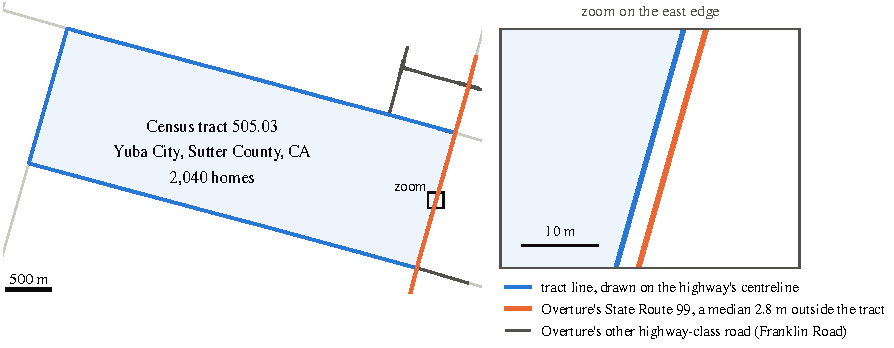
\includegraphics[width=\textwidth]{p2_worked_example.pdf}
\caption{Yuba City tract 505.03. The tract line and Overture's State Route~99 run side by side, a median 2.8~m apart, so
the reference counts a highway inside the tract that Overture places next door.}
\label{fig:example}
\end{figure*}

\section{Who is affected, and why it matters}
\label{sec:affected}
\textbf{In one sentence: the bookkeeping understates how far rural and fire-exposed places fall behind, invents most of
the reported gap for socially vulnerable ones, and sends a worklist to mapped highways in towns and cities while rural,
tribal and fire-exposed tracts wait.}

\subsection{It bends the scorecard built to reveal inequity}
\label{sec:scorecard}
The scorecard exists to show which people the map serves worse: it divides the mean score of rural, tribal, vulnerable or
hazard-exposed tracts by that of the rest. Table~\ref{tab:scorecard} and Figure~\ref{fig:scorecard} compute it on our
final submission twice: as scored,
which reproduces the card the leaderboard prints for that file, and with each highway counted once (a road-scored tract's
score loses the road gap the bookkeeping adds, divided by its three components). The bookkeeping is heaviest in towns and
cities, where highways run on tract lines and carry several route numbers, so it lifts urban scores and flattens the
comparisons. Counted once, rural tracts are 2.73 times as far behind as urban ones, not 2.34; on the road gap alone the
ratio doubles, from 1.67 to 3.32, and the tribal one rises from 2.98 to 5.23. The wildfire-hazard ratio rises from 1.67
to 1.81. In the other direction, the scorecard's social-vulnerability disparity (1.16) almost vanishes (1.01): nearly all
of it is bookkeeping in vulnerable urban tracts, not missing map. A reader of the official card would underrate the
disadvantage of exactly the rural and fire-exposed places that have the fewest alternatives when a road is wrong, and
would chase a social-vulnerability gap that is mostly an artefact.

\begin{table}[t]
\centering\small
\caption{The organisers' scorecard on our final submission (E136), as scored and with each highway counted once. Ratios
are the mean score of the first group over the second; median splits as in the scorecard.}
\label{tab:scorecard}
\footnotesize\setlength{\tabcolsep}{2.5pt}
\begin{tabular*}{\columnwidth}{@{\extracolsep{\fill}}lrrr@{}}
\toprule
Scorecard ratio & As scored & Counted once & Change\\
\midrule
Rural vs urban & 2.34 & \textbf{2.73} & +17\%\\
Wildfire hazard, high vs low & 1.67 & \textbf{1.81} & +9\%\\
Summer heat, high vs low & 0.59 & 0.64 & +10\%\\
Winter drought, high vs low & 1.30 & 1.32 & +2\%\\
Tribal vs non-tribal & 2.77 & 2.59 & $-$7\%\\
Climate vulnerability, high vs low & 1.40 & 1.27 & $-$9\%\\
Social vulnerability, high vs low & 1.16 & \textbf{1.01} & $-$13\%\\
\midrule
Road gap alone: rural vs urban & 1.67 & \textbf{3.32} & +99\%\\
Road gap alone: tribal vs non-tribal & 2.98 & \textbf{5.23} & +75\%\\
\bottomrule
\end{tabular*}
\end{table}

\subsection{A worklist built from the score points at mapped highways}
Road-coverage scores are the kind of number an emergency-management office or a mapping programme uses to decide where to
check evacuation routes, and where to add or verify highways before a fire, flood or hurricane season. Take the 660 tracts
with the worst road gap as that worklist. Half of it (321 tracts, 1.19 million people) is there because of counting
rules, and for those tracts the work would find nothing to fix: the highway is on the map, a few metres from the line.
Over the whole map, bookkeeping adds at least 0.2 to the road gap of 1,548 tracts, home to 5.8 million people, from the
Cheyenne and Arapaho and Cherokee tribal statistical areas of Oklahoma to Spokane, Yuba City, Woodland, San Angelo,
McAllen and Dallas. What they share is geometry: a highway on the tract's edge, or one that carries several route
numbers or names.

\subsection{Whose gaps it hides: rural, tribal and fire-exposed tracts}
Removing the bookkeeping does not only shrink gaps; it changes whose gaps they are. The 321 tracts that join the worst
tenth when each highway is counted once have a gap that is, by the score's own definition, mostly coverage: bookkeeping
is a median 29\% of their reference length, against 75\% in the tracts they would replace. Table~\ref{tab:hidden}
compares the two groups. The hidden tracts are 71\% rural, 58\% on tribal land and 83\% above the median wildfire hazard
potential, and half have burned since 1984. The tracts that crowd them out are 38\%, 26\%, 61\% and 11\%. So the score as
it stands ranks the places where a missing evacuation route is hardest to work around below places whose highways are
already on the map.

\begin{table}[t]
\centering\small
\caption{The two groups the bookkeeping swaps on a worst-tenth worklist. \emph{Hidden}: in the worst tenth only when
each highway is counted once. \emph{Mapped}: in it only as scored. Wildfire hazard is the package's USFS wildfire hazard
potential; burned is MTBS, 1984--2023; bookkeeping share is boundary plus duplicate length over the reference length.
Source: \code{numbers.json}, key \code{displaced}.}
\label{tab:hidden}
\setlength{\tabcolsep}{2.5pt}
\begin{tabular*}{\columnwidth}{@{\extracolsep{\fill}}lrrr@{}}
\toprule
 & Hidden & Mapped & All road-scored\\
\midrule
Tracts & 321 & 321 & 6,593\\
People (millions) & 1.00 & 1.19 & 27.1\\
Rural (RUCA $\geq$ 4) & \textbf{71\%} & 38\% & 24\%\\
On tribal land & \textbf{58\%} & 26\% & 11\%\\
Wildfire hazard above median & \textbf{83\%} & 61\% & 54\%\\
Burned since 1984 & \textbf{50\%} & 11\% & 13\%\\
Bookkeeping share (median) & 29\% & 75\% & 57\%\\
\bottomrule
\end{tabular*}
\end{table}

\begin{table}[t]
\centering\small
\caption{Six hidden tracts: rank by road gap among the 6,593 road-scored tracts, as scored and with each highway counted
once (the worst tenth is ranks 1--660). All six have burned since 1984.}
\label{tab:hiddennamed}
\footnotesize\setlength{\tabcolsep}{3pt}
\begin{tabularx}{\columnwidth}{@{}lLrr@{}}
\toprule
Tract (GEOID) & Where (tribal area) & People & Scored $\rightarrow$ once\\
\midrule
40085094300 & Love Co., OK (Chickasaw) & 2,023 & 665 $\rightarrow$ 30\\
40021977600 & Cherokee Co., OK (Cherokee) & 5,307 & 689 $\rightarrow$ 40\\
40029388200 & Coal Co., OK (Choctaw) & 1,702 & 1,063 $\rightarrow$ 48\\
48007950101 & Aransas Co., TX & 1,300 & 949 $\rightarrow$ 49\\
06103000100 & Tehama Co., CA & 4,670 & 1,139 $\rightarrow$ 50\\
40069660198 & Johnston Co., OK (Chickasaw) & 2,906 & 1,200 $\rightarrow$ 51\\
\bottomrule
\end{tabularx}
\end{table}

\subsection{What it means in named places}
\label{sec:named}
\paragraph{Yuba City, California (mapped, but flagged)} Tract 505.03 sits on State Route~99. In February 2017 the
Oroville spillway emergency led to the evacuation of about 188,000 people from Butte, Yuba and Sutter
counties~\cite{caloes}. The Sutter County grand jury then called for planned evacuation routes in a region with few ways
out, and found that opening a second lane on Highway 20 or 99 was seen as unrealistic~\cite{grandjury}. So Route~99 is a
road the region's evacuation planning depends on. The score marks this tract as missing three quarters of its highway,
yet Overture carries all 1,644~m of Route~99 along its edge (Figure~\ref{fig:example}). An agency checking evacuation
corridors by the score would spend its first visit on a road that is already mapped.

\paragraph{Aransas County, Texas (hidden)} Hurricane Harvey's centre came ashore in Aransas County in August 2017, near
Rockport and again west of Holiday Beach~\cite{harvey}. Tract 9501.01 there ranks 949th by road gap as scored and 49th
with each highway counted once: its gap is coverage, not counting, yet it sits outside a worst-tenth list.

\paragraph{Tribal Oklahoma and wildfire country (hidden)} Four of the six tracts in Table~\ref{tab:hiddennamed} lie in the
Chickasaw, Cherokee and Choctaw tribal statistical areas; all four have burned since 1984 and sit at or above the 70th
percentile of wildfire hazard among the challenge's tracts. The Tehama County tract is at the 99th percentile. These are
the places where a single missing or misclassified highway can decide how a community leaves ahead of a fire, and the
score as it stands ranks them below tracts whose highways are mapped.

\paragraph{Comparisons between places} A state agency comparing Oklahoma's urban road gap (0.32) with Arizona's (0.08)
would conclude that Oklahoma's highway map is four times less complete. Counted once, the two are 0.09 and 0.01. Most of
the difference is how often Oklahoma's highways run on tract lines and carry several names, not how well they are mapped.

\subsection{What public data outside the package say}
\label{sec:outside}
The prize form lets a discovery draw on public data beyond the package, so we asked two independent sources who lives in
the swapped tracts: the Census American Community Survey 2020--2024~\cite{acs} and FEMA's National Risk Index
v1.20~\cite{nri}. The package holds composite vulnerability indices but not these measures, and no scored file uses them
(Appendix~\ref{app:data}). We fixed twelve measures before computing any comparison, and we report all twelve
(Table~\ref{tab:outside}, Figure~\ref{fig:outside}).

\begin{table}[t]
\centering\small
\caption{The two groups of Table~\ref{tab:hidden} on public data outside the package. Shares are pooled over each group's
tracts; \emph{all} is every road-scored tract. FEMA \emph{high} means rated Relatively High or Very High. A higher
resilience score is better.}
\label{tab:outside}
\begin{tabularx}{\columnwidth}{@{}Lrrr@{}}
\toprule
Measure & Hidden & Flagged & All\\
\midrule
Homes that are mobile homes & 16.5\% & 9.3\% & 8.2\%\\
Households, no internet access & 11.3\% & 7.8\% & 6.8\%\\
People with a disability & 18.8\% & 15.3\% & 13.6\%\\
People aged 65 or over & 20.1\% & 17.4\% & 15.0\%\\
People below the poverty line & 15.3\% & 14.9\% & 13.9\%\\
Households, no vehicle & 4.1\% & 5.3\% & 5.5\%\\
\midrule
FEMA overall risk high, tracts & 41.4\% & 13.7\% & 20.9\%\\
FEMA wildfire risk high, tracts & 33.6\% & 11.2\% & 10.7\%\\
FEMA inland flood risk high, tracts & 34.3\% & 15.9\% & 26.4\%\\
FEMA annual loss per person & \$843 & \$451 & \$489\\
FEMA social vulnerability score & 69.3 & 58.2 & 55.7\\
FEMA community resilience score & 27.0 & 30.5 & 30.1\\
\bottomrule
\end{tabularx}
\end{table}

\begin{figure}[t]
\centering
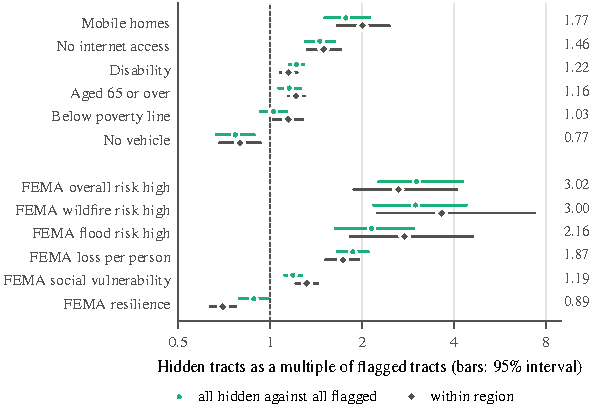
\includegraphics[width=\columnwidth]{p9_outside_check.pdf}
\caption{Hidden tracts against flagged tracts on all twelve measures; 1 means no difference, and the numbers on the right
are the pooled ratios. \emph{Within region} compares the groups inside each region, weighted by where the hidden tracts
are. Resilience is the one measure where lower means worse off.}
\label{fig:outside}
\end{figure}

Ten of the twelve point the same way, and all ten hold within regions. The hidden tracts have nearly twice the share of
mobile homes of the flagged tracts (16.5\% against 9.3\%), and more people aged 65 or over, more people with a disability
and more households with no internet access. FEMA rates three times as many of them high for wildfire risk (34\% against
11\%) and for overall risk (41\% against 14\%), and twice as many for inland flooding; it scores their community
resilience lower and expects nearly twice the annual loss per person (\$843 against \$451). Two measures do not follow
the pattern. Hidden tracts have fewer households with no vehicle (4.1\% against 5.3\%), so the bookkeeping does not hide
car-free households. Poverty is level overall (15.3\% against 14.9\%), and higher in hidden tracts only within regions.

In absolute terms the hidden tracts hold about 78,000 mobile homes, 189,000 people with a disability and 44,000 households
with no internet access. Two of these needs were named after Oroville: the Sutter County grand jury asked for plans for
people with disabilities and recorded concern that not everyone has internet access for emergency
information~\cite{grandjury}.

The bookkeeping also blunts the score as a guide to risk. Of the 706 road-scored tracts FEMA rates high for wildfire risk,
a worst-tenth worklist holds 110 as scored and 182 with each highway counted once; of the 1,742 rated high for inland
flooding, 139 and 198; of the 1,376 rated high overall, 130 and 219. The rank correlation between a tract's road gap and
FEMA's wildfire risk score rises from 0.33 to 0.45 (0.31 to 0.45 within regions). FEMA's index is built without this road
score, so this is an outside sign that taking the bookkeeping out points the road gap at the places with more to lose.

\section{Limits}
\label{sec:limits}
The split between bookkeeping and real coverage comes from our calibrated simulator, not from the hidden reference
itself, which is not in the package. The simulator's road part was tested against the hidden scores
(Figure~\ref{fig:agreement}), and Table~\ref{tab:sens} shows how far other weights move the share (55--80\%, or 46\% for
the boundary rule alone). The scorecard comparison of Table~\ref{tab:scorecard} uses our final submission as the best
available estimate of each tract's score, and removes the bookkeeping from a road-scored tract's score as one third of
its added road gap, which assumes the building and places components are defined (they are in almost every road-scored
tract). The leaderboard tests use the public 30\% of tracts, so their agreement values carry that sample's noise; the private 70\%, revealed after the close, backs the two rules that
can be read directly from it (the boundary rule took 0.08296 to 0.07708 from E18 to E19, and the re-measured boundary
distance 0.05790 to 0.05747 from E109 to E110). The hidden tracts of Table~\ref{tab:hidden} are those where the gap is \emph{not} bookkeeping; their remaining
gap rests largely on each region's calibrated ratio between the reference's road classes and Overture's, so the list
says where to look, not that a particular road is missing on the ground. And we cannot say how a given agency actually
uses the score; the worklist in Section~\ref{sec:affected} illustrates a use the score invites. Section~\ref{sec:outside}
describes groups of tracts, not people: Census figures are survey estimates, and FEMA describes its index as a nationwide
planning tool, not a substitute for local risk assessment. It shows who lives in the hidden tracts, not that their
highways are missing. The government reports cited in Section~\ref{sec:affected} give context only; no computed result
in this paper rests on them.

\section{What would fix it}
\label{sec:fix}
Three changes to the reference side would remove most of the effect: count a highway that lies on a tract boundary once,
on the side where it is mapped (or half on each side); remove duplicate records of the same geometry before measuring
length; and give both layers the same treatment of ramps (both include them, or neither does).

\section{Prior work}
\label{sec:prior}
Both counting mechanisms were first described by other participants, and we credit them here. A participant's post
``The road gap mostly measures TIGER's data model''~\cite{pio} makes the general claim first. Another participant's entry
``Counted twice: the score charges tracts for highways that run along their edge''~\cite{hhy} describes the boundary
mechanism and reports that modelling it improved their public score. A third participant's public method
notes~\cite{dante} state the duplicate-record
mechanism (the reference keeps one record per edge and name, so a road carrying two route numbers or a local street name
is counted again) and fit it on the leaderboard. Our contribution is to measure both from the package alone and test each
against the hidden scores (extending the record rule to honorific highway names, E97); to show that together they make up
72\% of the mean road gap, with duplicate records the larger part in every region; to show that the share differs by
region; and to trace the consequence for people: the rural, tribal and fire-exposed tracts the bookkeeping pushes down a
worklist, with named tracts and a worked example.

\partbanner{once}{Part B \quad Best Documentation: methodology}
\begin{tcolorbox}[enhanced,colback=white,colframe=once!60,boxrule=0.4pt,arc=1mm,left=1.5mm,right=1.5mm,top=0.8mm,bottom=0.8mm,
  title={\footnotesize\bfseries The method in five plain steps},coltitle=white,colbacktitle=once!85,toptitle=0.2mm,bottomtitle=0.2mm]
\footnotesize
\begin{enumerate}[leftmargin=1.2em,itemsep=1pt]
\item \textbf{Measure the map.} For every tract, lengths and counts from Overture's roads, places and buildings, and the
package's tables.
\item \textbf{Imagine the hidden reference.} A simulator draws, many times, how much reference road, how many facilities
and how many businesses each tract could have, applies the organisers' formula, and averages.
\item \textbf{Ask the leaderboard one question at a time.} Each idea goes up once as a small change to a scored file; two
scores give its agreement with the hidden target exactly.
\item \textbf{Combine without overfitting.} Package-only pieces are fitted to the shape of the best combination of scored
files, never to a score directly, and regularised for the private split.
\item \textbf{Correct what is left.} A seeded learner predicts the simulator's remaining error from the package; its
unmeasured part is the last step. Every final rebuilds from the package to $3\times10^{-16}$.
\end{enumerate}
\end{tcolorbox}

\section{Overview: predicting a score with no labels}
\label{sec:overview}
The challenge asks for a coverage-gap score for each of 9,794 census tracts in five regions (eastern Oklahoma, eastern
Washington, the Maricopa region of Arizona, northern California and south-central Texas). No tract-level labels exist.
The score compares Overture's roads, buildings and places with reference layers (TIGER/Line roads, Microsoft building
footprints, USGS/HIFLD facilities and County Business Patterns) that were removed from the package and that the rules
forbid us to use. So our model has to estimate, for each tract, how much reference road, how many reference buildings and
how many reference facilities and businesses there are, from what the package does contain, and then apply the
organisers' formula.

We did this with a simulator: for each tract it draws the hidden reference many times from distributions built on
Overture's own data, applies the scoring formula to each draw and averages the result. The simulator is calibrated to
published averages. Each new idea about how the reference behaves was added to our best file as a small change and
submitted once; the change in score measured how much the idea agrees with the hidden target. The final files combine
the measured ideas (Figure~\ref{fig:arch}). Our selected finals scored \finalAscore{} and \finalBscore{} on the public split and 0.056132715 and 0.05613082 on the private one; for
scale, predicting the mean everywhere scores 0.0890. Figure~\ref{fig:trajectory} shows how we got there.

\begin{figure}[t]
\centering
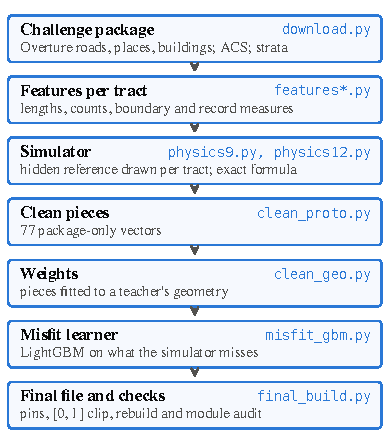
\includegraphics[width=0.94\columnwidth]{p7_architecture.pdf}
\caption{From the package to the final file; each box names the script that does it.}
\label{fig:arch}
\end{figure}

\section{Data sources}
\label{sec:data}
The scored submissions use only the challenge package~\cite{readme} (Table~\ref{tab:data}). External data appears nowhere
in them. Part~A goes outside the package once, in Section~\ref{sec:outside}, as the prize form allows, with the two public
datasets listed in Appendix~\ref{app:data}, and it cites three public reports for context.

\begin{table}[t]
\centering\small
\caption{Package layers used, and what we take from each.}
\label{tab:data}
\begin{tabularx}{\columnwidth}{@{}>{\raggedright\arraybackslash}p{0.30\columnwidth}L@{}}
\toprule
Layer & What we take from it\\
\midrule
Overture roads, release 2026-08-19.0~\cite{overture} & road length by class inside each tract; route numbers and names; ramps\\
Overture places & counts by category; names, confidence and source metadata\\
Overture buildings & footprint counts and sizes\\
Overture rail, infrastructure & rail lines (to set railway boundaries aside); transit stops\\
ACS housing (B25001) & housing units per tract\\
Tract polygons (TIGER 2025) & geometry, land area, population\\
Strata tables & urbanity (RUCA), tribal land, SVI, CVI, burned area, heat and drought\\
\bottomrule
\end{tabularx}
\end{table}

\section{How each component was computed}
\label{sec:components}
The score is the mean of the defined components; a component is undefined where the tract has no reference of that kind.
Each component is
\begin{equation*}
\text{gap} = 1-\min\!\left(1,\ \frac{\text{Overture amount}}{\text{reference amount}}\right).
\end{equation*}
We compute the Overture amount exactly as the organisers describe it and simulate the reference amount.

\paragraph{Roads} The Overture amount is the length of motorway, trunk, primary and secondary road inside the tract,
filtered on class only, as the organisers' text says (this keeps motorway ramps in). The reference amount is simulated as
a per-region scale times the bookkept reference length of Section~\ref{sec:pattern} (interior highway, plus boundary
highway, plus duplicate records, minus Arizona's route-log highway names, which are not reference records), with a
per-tract log-normal spread. The road component is defined where the bookkept length is positive; this reproduces the
organisers' published counts of road-undefined tracts to within 2\% per region (Arizona's exactly). The per-region scales
are calibrated to a competitor's published mean scores for 16 region, urbanity and burn cells (a published aggregate,
listed in \code{src/published.py}).

\paragraph{Facilities half of the places component} For fire stations, ambulance services and schools the Overture
amount is the count of places whose primary category is \code{fire\_department}, \code{ambulance\_and\_ems\_services} or
one of six school categories. The reference amount is the Overture count plus stations or schools the reference has and
Overture does not list under those categories: places filed under another category but named like a station or school,
stations traced only as buildings, one record per fire agency, and a background rate in tracts with no trace at all.
These rates are calibrated to two published counts (740 fire-station blackouts, 270 of them misfiled) and to the published
fire-to-school gap ratio.

\paragraph{Business half of the places component} The Overture amount is all places in the tract. The reference amount
(County Business Patterns establishments) is simulated from building counts, Overture's own record metadata and a wide
log-normal spread, scaled so the places component matches its published average of 0.052.

\paragraph{Buildings} The building gap is almost always near zero (Overture's footprints largely come from the same
machine-learned source as the reference), so it is a constant of 0.0065.

The simulator's mechanism weights (how fully boundary highways and duplicate names count, the rural station rate and so
on) were fitted to everything our scored files had revealed about the hidden target, then its prediction in the directions
no file had measured was submitted as a bet: a method we took from a participant's public notes~\cite{dante}. Its code is
\code{src/physics9.py}
(with \code{src/physics12.py} for the refits of 31 October); the fitted weights are committed in \code{params/}.

\section{Edge cases}
\label{sec:edge}
Table~\ref{tab:edge} lists every edge case the organisers name, and the rest we met. Two further rules keep files valid:
every file has 9,794 rows in the sample submission's order, with 11-character GEOIDs kept as text; and our writer refuses
to overwrite a file that has already been scored, because its score is the only measurement of that exact vector.

\begin{table}[t]
\centering\small
\caption{Edge cases and how each is handled.}
\label{tab:edge}
\begin{tabularx}{\columnwidth}{@{}>{\raggedright\arraybackslash}p{0.27\columnwidth}>{\raggedright\arraybackslash}p{0.17\columnwidth}L@{}}
\toprule
Case & Tracts & Handling\\
\midrule
Zero population & 27 (82 with no homes) & scored like any other tract; every ratio with a population or housing denominator is guarded\\
Water-dominated (zero land area) & 2 & no Overture road, building or place, so every defined component is $1-\min(1,0/\text{ref})=1$; set to exactly 1.0, later confirmed by a score change\\
Data-sparse: no Overture data at all & the same 2 & as above\\
Data-sparse: no Overture place of a type & 71\% fire, 93\% EMS, 21\% school & the simulator draws whether the reference holds one: gap 1 if it does, component undefined if not\\
Road component undefined & 3,201 & score is the mean of the places and building components\\
Eastern Washington & 415 & no published calibration; its road scale is the median of the other four regions'\\
Values outside $[0,1]$ & any & clipped to $[0,1]$ after combining\\
\bottomrule
\end{tabularx}
\end{table}

\section{How the final weights were set, and the alternatives we tried}
\label{sec:weights}
\paragraph{Measuring an idea with one submission} Each idea about the hidden reference was submitted once, as a small dose
$d$ on top of a scored base $b$. Because the score is an RMSE, two scores give the covariance of the change with the
target exactly: $\overline{d\,(y-b)} = \tfrac12\big(\overline{d^{2}} + \mathrm{MSE}_b - \mathrm{MSE}_{b+d}\big)$, where
the bars are means over the public tracts. Scaled by the dose's size, this is the idea's \emph{agreement} with the target
(Figure~\ref{fig:agreement}); its standard error over the 30\% public sample is about 0.02.

\paragraph{Building the finals} The finals are built in three steps. First, 77 package-only pieces (the simulator's variants
and the raw vectors of every idea we tested, rebuilt from the package) are fitted, by least squares and without using any
score, to reproduce the shape of a \emph{teacher}: a weighted combination of our scored files. Second, measured ideas are
added on top at their measured strength. Weighting by geometry rather than by score matters: when we let the scores choose
the pieces' weights directly, the fit exploited the noise of the 30\% public sample and the file scored 0.0016 worse than
predicted (E123 in Table~\ref{tab:weights}).

\paragraph{The misfit learner} Third, a learned correction. The part of the target the scored files already reveal is
known exactly (the teacher), and so is the simulator's projection on the same files; their difference is what the
simulator gets wrong, as far as the scores can see. A seeded LightGBM model (\code{src/misfit\_gbm.py}) learns that
difference from about 400 package features, out of fold (R$^2$ 0.45; the facility features matter most). Its prediction
in the directions no scored file has measured is the step: E134 added it to E132 and read an agreement of +0.030, the last
idea that paid. A better-fitting second version (R$^2$ 0.58) added nothing beyond it on the public score (E135), though it
later proved our best private file, and a refit of the simulator on all 104 scored files read +0.010 (E137), too small
to use, and scored worse than E136 on the private split (0.05623 against 0.05613).

\begin{table}[t]
\centering\small
\caption{Weightings and ideas tried in the last three days, and why each was kept or dropped. Scores are RMSE; every
decision used the public score, and private scores were revealed after the close
(\code{submissions/ledger.csv} lists every scored file; \code{docs/HISTORY.md} tells the whole story).}
\label{tab:weights}
\begin{tabularx}{\columnwidth}{@{}Lrr>{\raggedright\arraybackslash}p{0.21\columnwidth}@{}}
\toprule
Weighting or idea & Public & Private & Kept?\\
\midrule
Pieces weighted by their measured agreement (E123) & 0.05702 & 0.05773 & no: fitted the public sample's noise\\
Pieces fitted to our best earlier file's geometry (E124, 63 pieces) & 0.05631 & 0.05624 & superseded\\
Same with 77 pieces (E125) & 0.05582 & 0.05637 & superseded\\
Plus the fitted simulator's new part (E127) & 0.05576 & 0.05616 & yes, as a piece\\
Pieces fitted to a combination of 69 scored files (E129) & 0.05559 & 0.05617 & superseded\\
Same teacher, light regularisation (E131) & 0.05557 & 0.05615 & base of final B\\
Same teacher, stronger regularisation (E132) & 0.05563 & 0.05616 & base of final A\\
Housing term in the business reference (E130) & 0.05590 & 0.05629 & no: disagreed with the target\\
Vulnerability term in the business reference (E133) & 0.05567 & 0.05627 & no: carried no signal\\
Misfit learner's step on E132 (E134) & 0.05557 & 0.05613 & \textbf{final A}\\
Learner v2, beyond E134 (E135) & 0.05561 & 0.05610 & no: nothing new on public\\
E131 plus the learner's step at its optimum (E136) & 0.05551 & 0.05613 & \textbf{final B}\\
Simulator refit on all scored files (E137) & 0.05552 & 0.05623 & no: too small\\
\bottomrule
\end{tabularx}
\end{table}

\paragraph{Why two finals} Weights read from the public 30\% fit some of its noise, so a file tuned harder to the public
split does a little worse on the private 70\%. We simulated this with synthetic targets and the same file structure: a
teacher regularised more strongly gives up a little on the public split (0.00006 between E131 and E132) and should gain
about 0.0001 to 0.0002 on the private one. We selected one file of each kind, each with the learner's step: final A is
E132 plus the step (E134), final B is E131 plus the step at its measured optimum (E136). The private scores did not show
that gain: E132 scored 0.056156 against E131's 0.056149, and the two finals finished level at 0.056133 and 0.056131. The
learner's step did hold on the private split, taking E132 from 0.056156 to 0.056133. Our best private file was the
learner's second version, E135, at 0.056099, which we had set aside on its public score.

\begin{figure}[t]
\centering
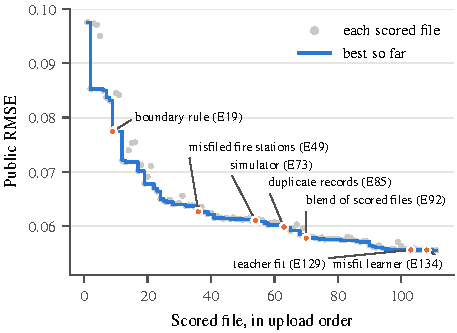
\includegraphics[width=\columnwidth]{p6_trajectory.pdf}
\caption{Public RMSE of every scored file, in upload order, with the discoveries that moved it most. Both finals scored
0.05613 on the private split (Table~\ref{tab:weights}). Early exploratory
files that we later excluded (Section~\ref{sec:excluded}) are included, so the curve is the history, not the finals.}
\label{fig:trajectory}
\end{figure}

\subsection{Validation: predicting a score before uploading it}
For a file that is a combination of scored files, the score can be predicted before uploading it from the files' own
scores and their second moments, by the identity above. We used the prediction to decide whether a file was worth a
submission (Table~\ref{tab:valid}). The predictions were within 0.0001, and the files did at least as well as predicted
when the pieces' weights were regularised as in E125, E129 and E132. E131, with weaker regularisation and chosen among many
variants, came in 0.00005 worse than predicted, and we changed the rule after it. Final B (E136) landed 0.0000025 better
than its prediction.

\begin{table}[t]
\centering\small
\caption{Predicted and actual public RMSE. We predicted public scores only; private scores are in Table~\ref{tab:weights}.}
\label{tab:valid}
\begin{tabular}{@{}lrr@{}}
\toprule
File & Predicted & Actual\\
\midrule
E125 & 0.05590 & 0.05582\\
E129 & 0.055590 & 0.055588\\
E131 & 0.05553 & 0.05557\\
E132 & 0.05565 & 0.05563\\
E136 & 0.055509 & 0.055506\\
\bottomrule
\end{tabular}
\end{table}

\section{Reproducing it}
\label{sec:repro}
Python 3.11 (\code{requirements.txt} pins every package), on Windows 11 or Linux, CPU only. Randomness is seeded: the
simulator uses seed 20261020 for every draw, the misfit learner seed 20261031 (deterministic LightGBM), and the early
files seed 20261011. The full sequence, with run times on our machine (Windows 11, 16~GB of memory), is in
Appendix~\ref{app:repro}. In short: download the package, build the per-tract features with one command (about 25
minutes), then \code{python src/final\_build.py NAME} rebuilds a final file from the package and the committed weights,
compares it with the uploaded CSV, and checks that no excluded module was loaded. Both finals rebuild to within
$3\times10^{-16}$ (E134 2.0e-16, E136 3.1e-16).

\subsection{What is not in the final files, and why}
\label{sec:excluded}
Early in the competition we built a few exploratory files that imposed another team's published table of mean scores at
full strength, or that adjusted our file to match the public scorecard printed beside the leaderboard's top entry. We
excluded those files and everything derived from them before building the finals: the finals are rebuilt from
package-only pieces, and \code{final\_build.py} stops with an error if the modules that did those things are loaded. The
published averages we do use (the 16 cell means as calibration targets for the road scale, the 740 and 270 fire-station
counts, the 0.052 places average, the fire-to-school ratio and the organisers' road-undefined counts) are listed with
their sources in \code{src/published.py}. They set a handful of constants; none is a per-tract value.

\subsection{Maintenance}
If Overture releases change, re-run the feature scripts and \code{final\_build.py}; the constants tied to published
numbers are all in \code{src/published.py}. If the strata tables change, only the urbanity and tribal definitions in
\code{src/strata.py} need checking. The simulator's fitted weights would need refitting only if the scoring formula changed.

\section{Conclusion}
As scored, most of the road gap is a property of the reference file's bookkeeping rather than of the map: a highway on a
tract line is counted on both sides, and a stretch with several route numbers or names is counted several times. The
effect is large, robust to how it is weighted, and uneven across places, so it does more than add noise: it bends the
scorecard built to reveal inequity, understating how far rural and fire-exposed places fall behind and manufacturing most
of the gap it reports for socially vulnerable ones. It can be removed on the reference side with the three changes of
Section~\ref{sec:fix}. Until it is, anyone who ranks places by the road score, or reads the scorecard's road-driven
disparities, should first subtract the boundary and duplicate-record lengths, which the challenge package alone is
enough to measure; the per-tract results we publish do this for every tract.

\begin{thebibliography}{9}\small\setlength{\itemsep}{1pt}
\bibitem{zindi} Zindi and Humane Intelligence. Bias Bounty Mapping Equity Challenge: overview, rules and evaluation.
\url{https://zindi.africa/competitions/bias-bounty-mapping-equity-challenge}.
\bibitem{readme} Humane Intelligence. Bias Bounty Mapping Equity Challenge data package and README. Source Cooperative,
2026. \url{https://source.coop/humane-intelligence/bias-bounty-mapping-equity-challenge}. Downloaded 10 October 2026.
\bibitem{mtfcc} U.S. Census Bureau. MAF/TIGER Feature Class Code definitions (S1100 primary road, S1200 secondary road).
\url{https://www.census.gov/library/reference/code-lists/mt-feature-class-codes.html}. Retrieved 31 October 2026.
\bibitem{garm} U.S. Census Bureau. Geographic Areas Reference Manual, Chapter~10: Census Tracts and Block Numbering
Areas. \url{https://www2.census.gov/geo/pdfs/reference/GARM/Ch10GARM.pdf}. Retrieved 31 October 2026.
\bibitem{overture} Overture Maps Foundation. Overture Maps data, release 2026-08-19.0. \url{https://overturemaps.org}.
\bibitem{pio} Challenge participant. ``Bias discovery: the road gap mostly measures TIGER's data model, and hides where
Oklahoma's tribal nations are actually under-mapped.'' Challenge discussion 35000, 25 September 2026.
\url{https://zindi.africa/competitions/bias-bounty-mapping-equity-challenge/discussions/35000}.
\bibitem{hhy} Challenge participant. ``Entry for Best Bias Discovery, submission LJCWP9VU: Counted twice: the score
charges tracts for highways that run along their edge.'' Challenge discussion 35478, 21 October 2026.
\url{https://zindi.africa/competitions/bias-bounty-mapping-equity-challenge/discussions/35478}.
\bibitem{dante} Challenge participant. Public method notes (METHOD.md, \texttt{dev} branch), 22 October 2026.
\url{https://github.com/iam-dante/bias-bounty-competition}. Retrieved 31 October 2026.
\bibitem{caloes} California Governor's Office of Emergency Services. 2017 February Oroville Spillway Incident: After
Action/Corrective Action Report. November 2019.
\url{https://www.caloes.ca.gov/wp-content/uploads/Preparedness/Documents/2017-Oroville-Dam-Incident-AAR-Approved.pdf}.
Retrieved 31 October 2026.
\bibitem{grandjury} Sutter County Grand Jury. Emergency Evacuation Report, in the 2016--2017 Final Report, filed 30 June
2017. \url{https://www.sutter.courts.ca.gov/system/files?file=final-report-2016-2017-sutter-county-grand-jury-filed-06-30-17.pdf}.
Retrieved 31 October 2026.
\bibitem{harvey} E.~S. Blake and D.~A. Zelinsky. National Hurricane Center Tropical Cyclone Report: Hurricane Harvey
(AL092017). 9 May 2018. \url{https://www.nhc.noaa.gov/data/tcr/AL092017_Harvey.pdf}. Retrieved 31 October 2026.
\bibitem{acs} U.S. Census Bureau. American Community Survey 2020--2024 5-year detailed tables B01001, B17001, B18101,
B25024, B25044 and B28002, table-based summary file.
\url{https://www2.census.gov/programs-surveys/acs/summary_file/2024/table-based-SF/data/5YRData/}. Retrieved 31 October
2026, 16:27 UTC.
\bibitem{nri} Federal Emergency Management Agency. National Risk Index, census tracts, version 1.20, December 2025.
\url{https://services.arcgis.com/XG15cJAlne2vxtgt/arcgis/rest/services/National_Risk_Index_Census_Tracts/FeatureServer/0}.
Retrieved 31 October 2026, 16:27 UTC. Listed as a U.S. Government Work at
\url{https://catalog.data.gov/dataset/national-risk-index-nri-data}.
\end{thebibliography}

\newpage
\appendix
\section{Reproducing every number}
\label{app:repro}
Every command runs from the repository root with \code{python} (Python 3.11).
\begin{table}[H]
\centering\footnotesize
\begin{tabularx}{\columnwidth}{@{}>{\raggedright\arraybackslash}p{0.22\columnwidth}Lr@{}}
\toprule
Step & Command & Time\\
\midrule
Quick check of Part A & \texttt{src/download.py --strata}, then \texttt{src/quick\_check.py} & 1 min\\
Download the package & \texttt{src/download.py} & 40 min\\
Features per tract & \texttt{src/build\_features.py} (every builder, in order) & 25 min\\
Rebuild final B & \texttt{src/final\_build.py e136\_finalB} (rebuilds E131, E132, E134) & 10 min\\
Rebuild final A & \texttt{src/final\_build.py e134\_learner} & 8 min\\
Part A numbers & \texttt{src/writeup\_numbers.py}, then with \texttt{displaced}, \texttt{scorecard}, \texttt{sensitivity} & 5 min\\
Outside check, Section~\ref{sec:outside} & \texttt{src/external\_context.py} (add \texttt{fetch} to download again) & 1 min\\
Figures & \texttt{src/paper\_figures.py} & 1 min\\
This PDF & \texttt{pdflatex paper.tex} (twice), in \texttt{docs/paper} & 1 min\\
\bottomrule
\end{tabularx}
\end{table}
\Needspace{7\baselineskip}
{\raggedright Expected outputs (the download time assumes about 3~MB/s):
\begin{itemize}
\item \code{docs/writeup/numbers.json}, with \code{road\_gap\_mean} = \{as\_scored 0.166, counted\_once 0.047\} and
\code{added\_ge\_0.2\_total.tracts} = 1548;
\item \code{docs/writeup/worked\_example.json}, with \code{route\_highway\_along\_edge\_m} = 1643.5.
\end{itemize}\par}

\section{Data sources and licences}
\label{app:data}
All data behind the scored files and Sections~\ref{sec:pattern} to~\ref{sec:named} come from the challenge package on Source Cooperative~\cite{readme}, downloaded on 10 October 2026 (the package
version without the removed layers): Overture Maps release 2026-08-19.0~\cite{overture} (roads, buildings and rail under
ODbL; places and infrastructure under CDLA-Permissive~2.0; \textcopyright{} Overture Maps Foundation and its sources,
including OpenStreetMap contributors), Census TIGER/Line 2025 tract geometry and ACS 2020--2024 housing units (public
domain), and the strata tables listed in the package README under their own licences. No external data enters any
scored file.

\paragraph{Outside the package (Section~\ref{sec:outside} only)} Both sources are public and need no account or key.
Adding \code{fetch} to \code{external\_context.py} downloads them again; our extract for the 9,794 tracts is
\code{external\_tracts.csv} in \code{docs/writeup/}. The ACS tables~\cite{acs} are U.S. Census Bureau data in the public domain.
FEMA's index~\cite{nri} is listed on data.gov as a U.S. Government Work and carries FEMA's terms, which ask for this
statement: This product uses the Federal Emergency Management Agency's National Risk Index dataset API or downloadable
datasets but is not endorsed by FEMA. The Federal Government or FEMA cannot vouch for the data or analyses derived from
these data after the data have been retrieved from the Agency's website(s).

Section~\ref{sec:affected} also cites three government reports for context, each with its URL and retrieval date in the
references~\cite{caloes,grandjury,harvey}.

\section{Glossary}
\begin{description}[leftmargin=0pt,itemsep=1pt,font=\normalfont\bfseries,before={\interlinepenalty=10000 \widowpenalty=10000 \clubpenalty=10000}]
\item[Bookkept reference length] the reference road length a tract receives under the organisers' overlay, including
boundary highways and duplicate records.
\item[Boundary highway] a highway whose centreline is the tract line.
\item[Duplicate record] an extra reference record on the same stretch of road for a second route number or name.
\item[Agreement with the hidden target] the covariance between a change and the target, read from the score change and
scaled like a correlation.
\item[Road-scored tract] a tract whose road component is defined.
\item[Simulator] our model that draws the hidden reference and applies the scoring formula.
\item[Teacher] a combination of scored files whose shape the package-only pieces are fitted to.
\end{description}

\section{Submissions and use of AI tools}
Selected finals: \code{\finalAid} (\finalAname, public RMSE \finalAscore, private 0.056132715) and \code{\finalBid} (\finalBname, public RMSE
\finalBscore, private 0.05613082). We used an LLM
coding assistant for code drafting, debugging and editing this document. Every analysis, number and claim was checked by
the team, and the pipeline runs without it.

\end{document}
